\documentclass{article}
\usepackage{arxiv}

\usepackage[utf8]{inputenc}
\usepackage[english, russian]{babel}
\usepackage[T1]{fontenc}
\usepackage{url}
\usepackage{booktabs}
\usepackage{amsfonts}
\usepackage{nicefrac}
\usepackage{microtype}
\usepackage{lipsum}
\usepackage{graphicx}
\usepackage{natbib}
\usepackage{doi}
\usepackage{float}
\usepackage{caption}


\title{Порождающие модели для прогнозирования (наборов временных рядов) в метрическом вероятностном пространстве}

\author{ Карпеев Глеб \\
% \thanks{Use footnote for providing further
% 		information about author (webpage, alternative
% 		address)---\emph{not} for acknowledging funding agencies.} \\
	Кафедра интеллектуальных систем\\
	МФТИ\\
	% Pittsburgh, PA 15213 \\
	\texttt{karpeev.ga@phystech.edu} \\
	%% examples of more authors
	\And
	Vadim Strijov \\
	FRC CSC of the RAS\\
	Moscow, Russia\\
        \texttt{strijov@phystech.edu} \\
        \And
	Яковлев Константин \\
	Кафедра интеллектуальных систем\\
	МФТИ\\
	\texttt{iakovlev.kd@phystech.edu} \\
	% Santa Narimana, Levand \\
	% \texttt{stariate@ee.mount-sheikh.edu} \\
	%% \AND
	%% Coauthor \\
	%% Affiliation \\
	%% Address \\
	%% \texttt{email} \\
	%% \And
	%% Coauthor \\
	%% Affiliation \\
	%% Address \\
	%% \texttt{email} \\
	%% \And
	%% Coauthor \\
	%% Affiliation \\
	%% Address \\
	%% \texttt{email} \\
}
\date{}

\renewcommand{\shorttitle}{\textit{arXiv} Template}

%%% Add PDF metadata to help others organize their library
%%% Once the PDF is generated, you can check the metadata with
%%% $ pdfinfo template.pdf
\hypersetup{
pdftitle={A template for the arxiv style},
pdfsubject={q-bio.NC, q-bio.QM},
pdfauthor={David S.~Hippocampus, Elias D.~Striatum},
pdfkeywords={First keyword, Second keyword, More},
}

\begin{document}
\maketitle

\begin{abstract}
	Исследование посвящено проблеме прогнозирования временных рядов с высокой ковариацией. Задача решается для наборов временных рядов с высокой дисперсией, проявляющейся, например, в сигналах головного мозга или ценах финансовых активов. Для решения данной задачи предлагается построение пространства парных расстояний, представляющего метрическую конфигурацию временных рядов. Прогноз осуществляется в данном пространстве, а затем результат возвращается в исходное пространство с использованием метода многомерного шкалирования. В данной работе изучаются порождающие модели для прогнозирования наборов временных рядов в метрическом вероятностном пространстве. Новизна работы заключается в применении Римановых моделей для регрессии и использовании Римановых генеративных диффузных моделей.

\end{abstract}


\keywords{Riemannian Generative Models \and Trades}

\section{Introduction}
Развитие технологий, которое мы наблюдаем в последние годы, открывает перед нами широкие возможности для получения данных, передаваемых человеком с помощью различных устройств. Анализ данных систем, предназначенных для мониторинга состояния человека, позволяет решать задачи в сфере здравоохранения, которые включают в себя анализ сигналов головного мозга [1], мониторинга физической активности [2]. Задача прогнозирования временного ряда является важной частью анализа сигналов и может использоваться во многих биомедицинских приложениях.

В данной работе предлагается метод прогнозирования временных рядов с высокой ковариацией и высокой дисперсией. Предлагаемое решение задачи прогнозирования состоит из трех этапов. Во-первых, осуществляется построение пространства парных расстояний, где используемая метрика удовлетворяет условию Мерсера. Во-вторых, выполняется прогноз матрицы попарных расстояний. В-третьих, результат возвращается в исходное пространство.  В данной работе изучаются Римановы генеративные диффузные модели (RSGMs) [3] для выполнения прогнозирования матрицы попарных расстояний.


Классическими алгоритмами прогнозирования временных рядов являются метод SSA (Singular Spectrum Analysis) [4], LSTM [5], State space model [6]. Новизна предложенного метода заключается в том, что выполняется кодирование временных рядов с помощью матрицы расстояний, выполняется прогноз, а затем декодирование полученной матрицы.

Анализ предлагаемого метода прогнозирования проводится на синтетических и реальных данных. Синтетический набор данных построен на основе синусоидальных сигналах со случайной амплитудой и частотой. Реальные данные были получены с помощью акселерометра, а так же на основе финансовых временных рядов. Целью эксперимента является нахождение оптимальной модели для прогнозирования временных рядов.

\section{Problem Statement}
\label{sec:headings}

Даны временные ряды с высокой ковариацией и высокой дисперсией

% See Section \ref{sec:headings}.

\begin{equation}
	x_1, x_2, \ldots, x_T \in \mathbb{R}^d,
\end{equation}

где $d$ — количество временных рядов.

Нужно спрогнозировать $x_{T+1}$.

Алгоритм:

1. Построить матрицу расстояний.

\begin{equation}
\hat{\Sigma}_T = \frac{1}{T} \sum_{t=1}^{T} (x_t - \mu_T)(x_t - \mu_T)^T
\end{equation}

\begin{equation}
\mu_T = \frac{1}{T} \sum_{t=1}^{T} x_t
\end{equation}

2. Спрогнозировать матрицу $\hat{\Sigma}_{T+1}^s \approx \hat{\Sigma}_{T+1} | \hat{\Sigma}_{T}$

Базовый алгоритм - линейная регресиия:

\begin{equation}
\hat{\Sigma}_{T+1}^s = W \cdot \hat{\Sigma}_{T}
\end{equation}


3. Найти такой оптимальный $x_{T+1}$, что ошибка прогнозирования временных рядов

\begin{equation}
    \| \hat{\Sigma}_{T+1}^s - \hat{\Sigma}_{T+1} \|_2 \to \min_{\underset x_{T+1}}
\end{equation}



% \subsubsection{Headings: third level}
% \lipsum[6]

% \paragraph{Paragraph}
% \lipsum[7]


\section{Computation experiment}

Эксперимент проводился на реальных и синтетических данных. Синтетический набор данных построен на основе синусоидальных сигналах со случайной амплитудой и частотой. Реальные данные были получены с энергетической биржи Nord Pool [8] и представляют собой временной ряд цены на электроэнергию. Временной ряд энергии состоит из почасовых записей (всего 50826 наблюдений). 

Для оценивания качества аппроксимации вычисляется значение среднеквадратичной ошибки.

\begin{equation}
MSE(y_{pred}, y_{true}) = \frac{1}{n} \sum_{i=1}^n (y_{pred} - y_{true})^2
\end{equation}

Сравним два базовых алгоритма предсказания временных рядов - SSA и MSSA.

\subsection{Синтетические данные}

Сгенерируем выборку из двух синусоидальных сигналов размера $N = 200$, с количеством периодов 2 и 4, соответственно. Предскажем последние 40 значений выборки, для предсказания будем использовать последние 60 сгенерированных значений.\\

\begin{figure}[H]
    \begin{subfigure}
	\centering
	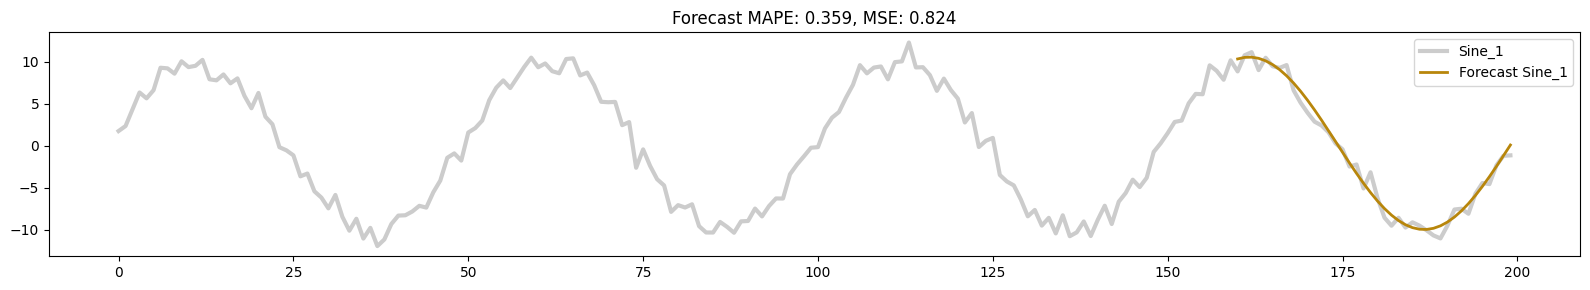
\includegraphics[width=1\textwidth]{figures/ssa_sin_low_noise.png}
	\caption{Прогноз синуса с 4 периодами алгоритмом SSA}
	\label{fig:fig2}
    \end{subfigure}

    \vspace{\baselineskip}

    \begin{subfigure}
	\centering
	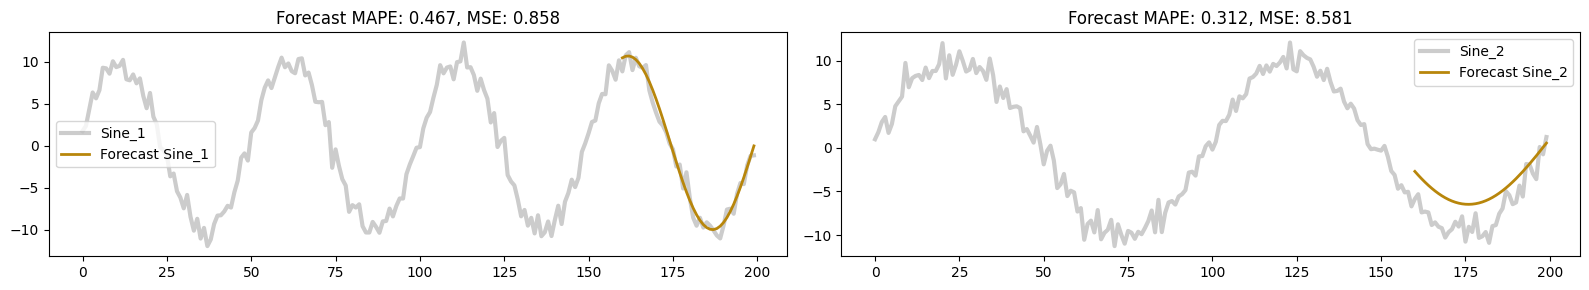
\includegraphics[width=1\textwidth]{figures/mssa_2sin_low_noise.png}
	\caption{Прогноз синуса с 2 и 4 периодами алгоритмом MSSA}
	\label{fig:fig2}
    \end{subfigure}

    \vspace{\baselineskip}

    \begin{subfigure}
	\centering
	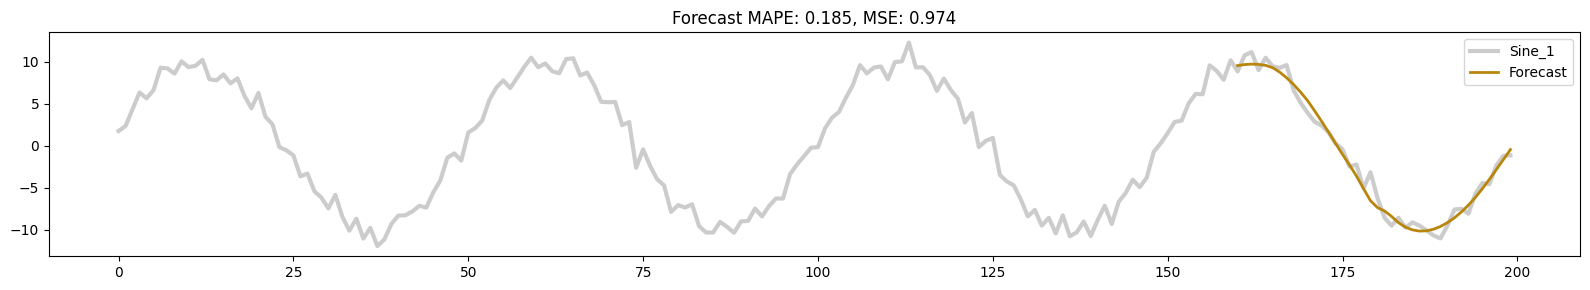
\includegraphics[width=1\textwidth]{figures/lstm_sin_low_noise.png}
	\caption{Прогноз синуса с 4 периодами алгоритмом LSTM}
	\label{fig:fig2}
    \end{subfigure}

    \vspace{\baselineskip}

    \begin{subfigure}
	\centering
	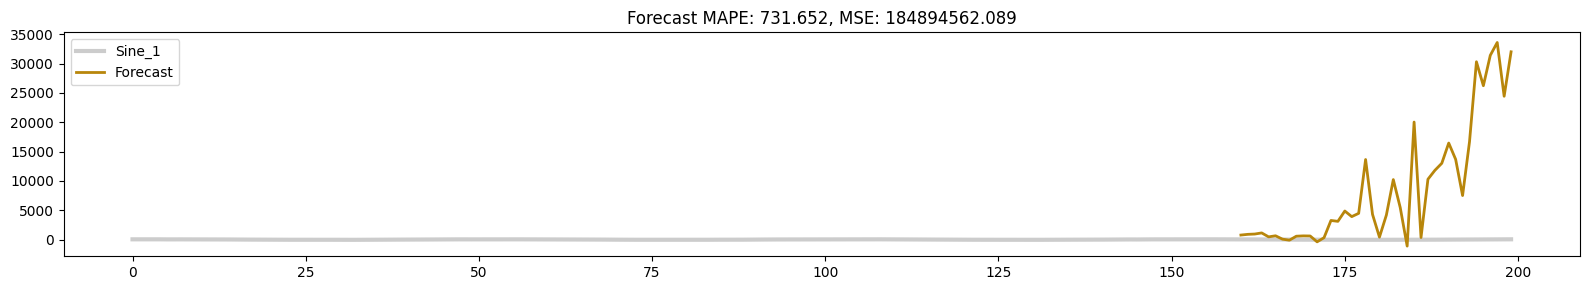
\includegraphics[width=1\textwidth]{figures/lstm_sin_high_noise.png}
	\caption{Прогноз сильно зашумленного синуса с 4 периодами алгоритмом LSTM}
	\label{fig:fig2}
    \end{subfigure}

    \vspace{\baselineskip}

    \begin{subfigure}
	\centering
	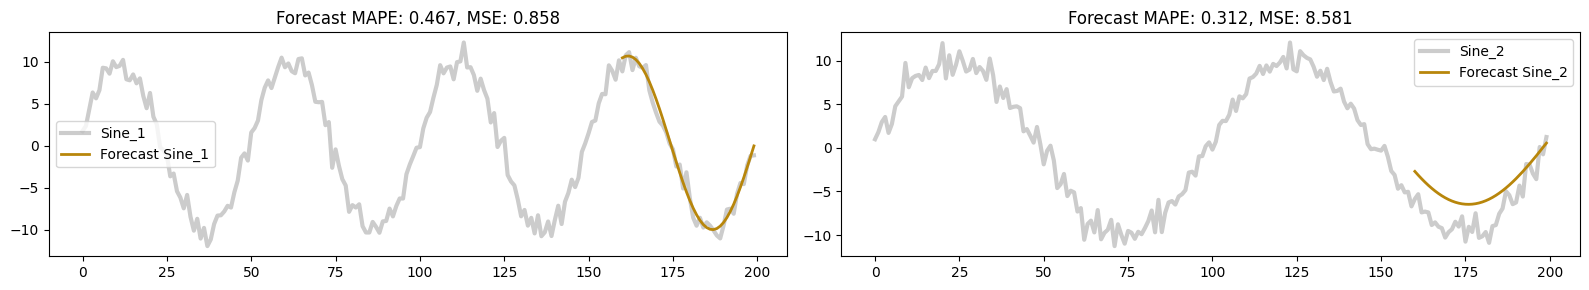
\includegraphics[width=1\textwidth]{figures/mssa_2sin_high_noise.png}
	\caption{Прогноз сильно зашумленного синуса с 2 и 4 периодами алгоритмом MSSA}
	\label{fig:fig2}
    \end{subfigure}
\end{figure}

% Видно, что восстановленный ряд получился примерно одинаковый.
\subsection{Данные цен на электроэнергию}

Строка матрицы $X$ –– локальная история сигнала за одну неделю $n = 24 \times 7$. Строка матрицы
$Y$ — локальный прогноз потребления электроэнергии в следующие 24 часа. Прогноз выполняется с помощью алгоритма SSA.

\begin{figure}[H]
	\centering
	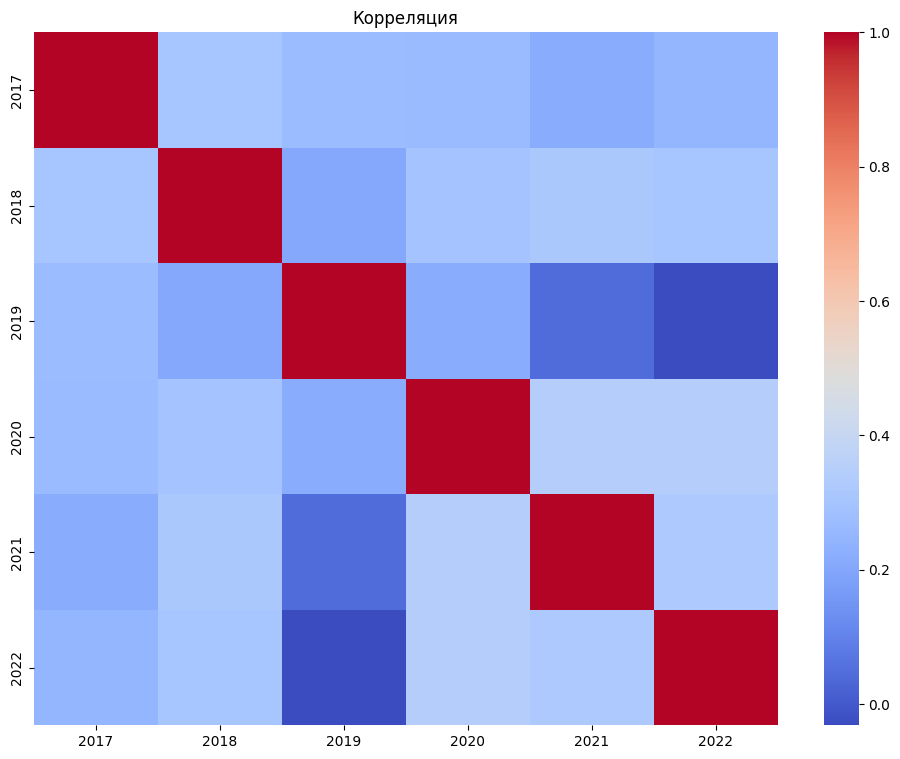
\includegraphics[width=0.6\textwidth]{figures/correlation_elspots.png}
	\caption{Корреляция между временными рядами}
	\label{fig:fig3}
\end{figure}

\begin{figure}[H]
	\centering
	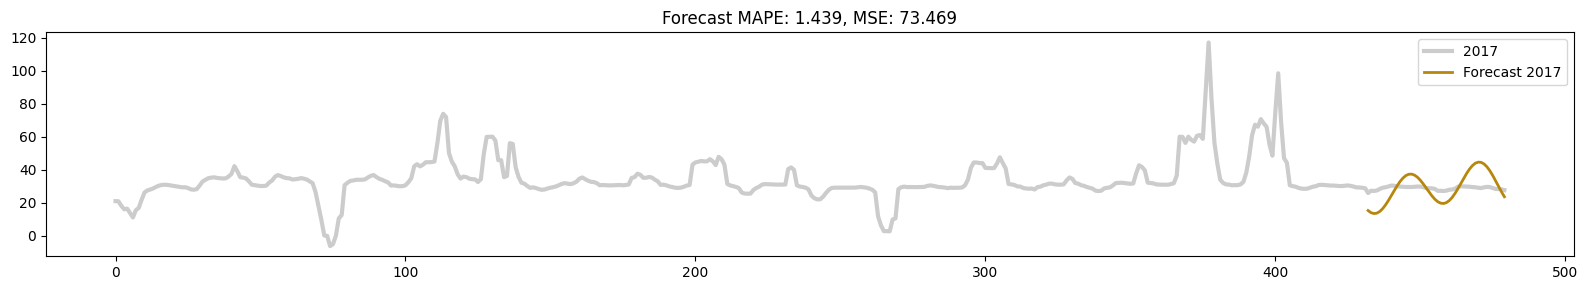
\includegraphics[width=0.75\textwidth]{figures/ssa_elspot_2017_plot.png}
	\caption{Прогноз спотовых цен на электроэнергию алгоритмом SSA}
	\label{fig:fig3}
\end{figure}

\begin{figure}[H]
	\centering
	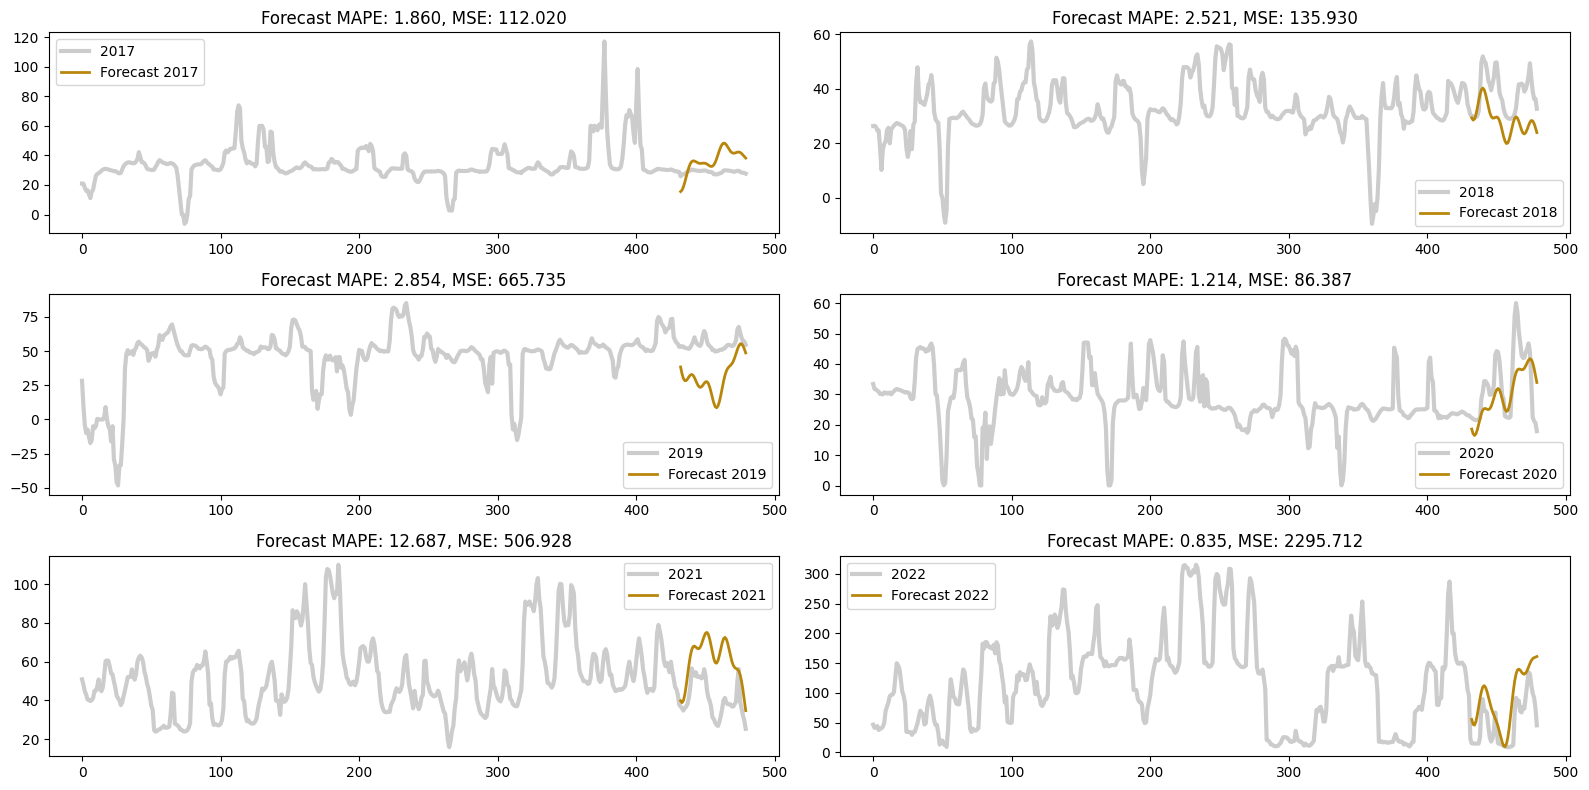
\includegraphics[width=1\textwidth]{figures/mssa_elspot_6plots.png}
	\caption{Прогноз спотовых цен по годам на электроэнергию алгоритмом MSSA}
	\label{fig:fig3}
\end{figure}

\begin{figure}[H]
	\centering
	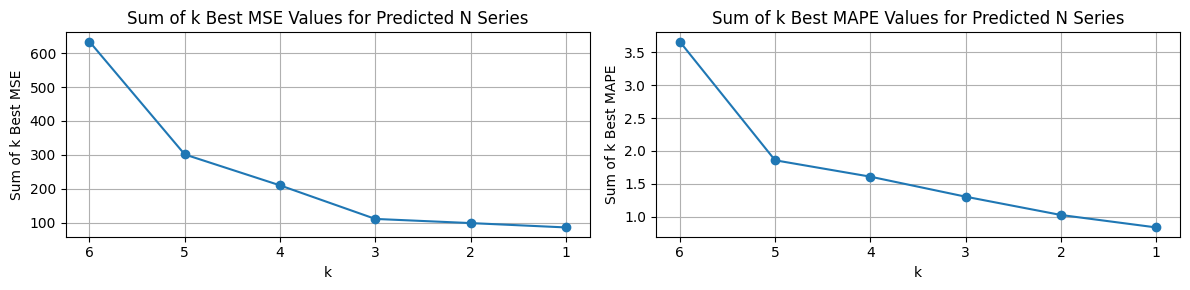
\includegraphics[width=1\textwidth]{figures/optimal_front.png}
	\caption{Pareto front для MSSA прогноза}
	\label{fig:fig3}
\end{figure}
% \section{Examples of citations, figures, tables, references}
% \label{sec:others}

% \subsection{Citations}
% Citations use \verb+natbib+. The documentation may be found at
% \begin{center}
% 	\url{http://mirrors.ctan.org/macros/latex/contrib/natbib/natnotes.pdf}
% \end{center}

% Here is an example usage of the two main commands (\verb+citet+ and \verb+citep+): Some people thought a thing \citep{kour2014real, hadash2018estimate} but other people thought something else \citep{kour2014fast}. Many people have speculated that if we knew exactly why \citet{kour2014fast} thought this\dots

% \subsection{Figures}
% \lipsum[10]
% See Figure \ref{fig:electricity_prediction.png}. Here is how you add footnotes. \footnote{Sample of the first footnote.}
% \lipsum[11]

% \begin{figure}
% 	\centering
% 	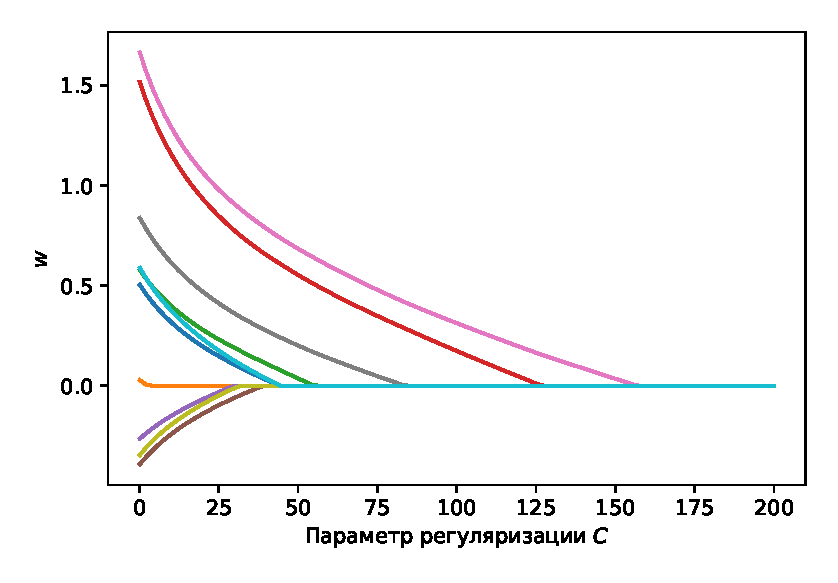
\includegraphics[width=0.5\textwidth]{../figures/log_reg_cs_exp.eps}
% 	\caption{Sample figure caption.}
% 	\label{fig:fig1}
% \end{figure}

% \subsection{Tables}
% See awesome Table~\ref{tab:table}.

% The documentation for \verb+booktabs+ (`Publication quality tables in LaTeX') is available from:
% \begin{center}
% 	\url{https://www.ctan.org/pkg/booktabs}
% \end{center}


% \begin{table}
% 	\caption{Sample table title}
% 	\centering
% 	\begin{tabular}{lll}
% 		\toprule
% 		\multicolumn{2}{c}{Part}                   \\
% 		\cmidrule(r){1-2}
% 		Name     & Description     & Size ($\mu$m) \\
% 		\midrule
% 		Dendrite & Input terminal  & $\sim$100     \\
% 		Axon     & Output terminal & $\sim$10      \\
% 		Soma     & Cell body       & up to $10^6$  \\
% 		\bottomrule
% 	\end{tabular}
% 	\label{tab:table}
% \end{table}

% \subsection{Lists}
% \begin{itemize}
% 	\item Lorem ipsum dolor sit amet
% 	\item consectetur adipiscing elit.
% 	\item Aliquam dignissim blandit est, in dictum tortor gravida eget. In ac rutrum magna.
% \end{itemize}


\bibliographystyle{unsrtnat}
\bibliography{references}

[1] S. Vaid, P. Singh and C. Kaur, "EEG Signal Analysis for BCI Interface: A Review, 2015 Fifth International Conference on Advanced Computing \& Communication Technologies, Haryana, India, 2015 \\

[2] Amit Purwar, Do Un Jeong and Wan Young Chung, "Activity monitoring from real-time triaxial accelerometer data using sensor network," 2007 International Conference on Control, Automation and Systems, Seoul, Korea (South), 2007 \\

[3] Riemannian Score-Based Generative Modelling. 
Valentin De Bortoli, Émile Mathieu, Michael Hutchinson, James Thornton, Yee Whye Teh, Arnaud Doucet, 2022 \\

[4] Elsner, J.B. and Tsonis, A.A. (1996): Singular Spectrum Analysis. A New Tool in Time Series Analysis, Plenum Press. \\

[5] Hochreiter, Sepp \& Schmidhuber, Jürgen. (1997). Long Short-term Memory. Neural computation. \\

[6] Koller D, Friedman N. (2009) Probabilistic Graphical Models. Cambridge, MA: MIT Press. \\

[7] Dataset for "Trades Quotes and Prices" \\

[8] Electricity Spot Price Data. 
https://www.kaggle.com/datasets/arashnic/electricity-spot-price \\

% [4] Introduction to Probabilistic Programming by A. Das, 2020 \\

% [5] Foundation of Variational Autoencoder (VAE) by A. Das, 2020 \\

% [6] From Autoencoder to Beta-VAE by L. Weng, 2018 \\

% [7] Flow-based Deep Generative Models by L. Weng, 2018 \\

% [8] Normalizing Flows: review by I. Kobyzin et al., 2020 \\

% [9] Variational Inference with Normalizing Flows by D.J. Rezende, S.
% Mohamed, 2015 \\

% [10] Score-Based Generative Modeling through Stochastic Differential
% Equations by Y. Song et al., 2015 \\

% [11] Denoising diffusion probabilistic models by J. Ho, 2020 \\

% [12] Deep unsupervised learning using Nonequilibrium Thermodynamics by
% J. Sohl-Dickstein et al., 2015 \\

% [13] An Intuitive Tutorial to Gaussian Processes Regression by J. Wang,
% 2020 \\

% [14] Extracting fundamental periods to segment biomedical signals
% Anastasia Motrenko, Vadim Strijov \\

% [15] Quasi-periodic time series clustering for human activity recognition
% A. V. Grabovoy, V. V. Strijov \\

% [16] Selection of superposition of models for railway freight forecasting
% N. D. Uvarov, M. P. Kuznetsov, A. S. Malkova, K. V. Rudakov , V. V. Strijov \\

% [17] Dynamic Trading with Predictable Returns and Transaction Costs
% N Garleanu \\

\end{document}